\documentclass{school-22.101-notes}
\date{October 12, 2011}

\begin{document}
\maketitle

\subtopic{Case 1, $\ddt \expect{x}, \hat{H} = \frac{\hat{p}^2}{2m} + V(x) $}

\begin{align}
\ddt \expect{x} &= \frac{i}{\hbar} \expect{\left[ \hat{H}, \hat{x} \right]} \\
&= \frac{i}{\hbar} \expect{\left[ \frac{\hat{p}^2}{2m} + V(x), \hat{x} \right]} \\
&= \frac{i}{\hbar} \expect{\left[ \frac{\hat{p}^2}{2m} , \hat{x} \right]} \\
&= \frac{i}{2m\hbar} \expect{\left[ \hat{p}^2 , \hat{x} \right]} \\
&= \frac{i}{2m\hbar} (-2i\hbar \hat{p} ) \\
&= \boxed{\frac{1}{m} \expect{p}}
\end{align}

\subtopic{Case 2, $\ddt \expect{p}, \hat{H} = \frac{\hat{p}^2}{2m} + V(x) $}

\begin{align}
\ddt \expect{p} &= \frac{i}{\hbar} \expect{\left[ \hat{H}, \hat{p} \right]} \\
&= \frac{i}{\hbar} \expect{\left[ \frac{\hat{p}^2}{2m} + V(x), \hat{p} \right]} \\
&= \frac{i}{\hbar} \expect{\left[ V(x) , \hat{p} \right]} \\
&= \frac{i}{\hbar} \expect{\left[ V(x), - i\hbar \ppx \right]} \\
&= \frac{i}{\hbar} \expect{(-i\hbar) (V(x) \ppx - \ppx V(x))} \\
&= \frac{i}{\hbar} \expect{i\hbar\pVpx} \\
&= \boxed{- \expect{\pVpx}}
\end{align}
This is called Ehrenfest's Principle, which is a quantum mechanical equation for average/expectation values of p(t). 

\lecture{Angular Momentum}
Angular momentum is a conserved quantity in a central force field. While a general potential is dependent on the spatial coordinate:
\eqn{ V(\uline{x}) = V(r,\theta, \phi)   }
a special potential that is only depend on radius (no $\theta, \phi$ dependency) is called a central force field because of its rotational symmetry. 


\topic{Orbital Angular Momentum}
This is similar to its classical description of angular momentum. 

\subtopic{Construct Cartesian Components of $\hat{L}$}
We define the orbital angular momentum like:
\begin{align}
\hat{\uline{L}} &= \hat{\uline{r}} \cross \hat{\uline{p}} \\
\hat{\uline{L}}_x &= \hat{y} \hat{p}_z - \hat{z} \hat{p}_y = - i\hbar \left( y \ppz - z \ppy \right) \\
\hat{\uline{L}}_y &= \hat{z} \hat{p}_x - \hat{z} \hat{p}_x = - i\hbar \left( z \ppx - x \ppz \right) \\
\hat{\uline{L}}_z &= \hat{x} \hat{p}_y - \hat{y} \hat{p}_x = - i\hbar \left( x \ppy - y \ppx \right) 
\end{align}

\subtopic{Check the Components We Just Constructed}
The question we want to ask is, `can we find the eigenvalues of each of the operators simultaneously?'

To answer the above question, we consider whether the components commute with each other. Because if $\left[ \hat{L}_x, \hat{L}_y \right] = 0$, that is to say we can pin $L_x, L_y$ at the same time. 

Though when we derive it for real (see notes), they come out to be:
\eqn{ \left[ \hat{L}_x, \hat{L}_y \right] = i \hbar ( \hat{x} \hat{P}_y - \hat{y} \hat{P}_x) = i\hbar \hat{L}_z }
\eqn{ \left[ \hat{L}_y, \hat{L}_z \right] = i \hbar ( \hat{y} \hat{P}_z - \hat{z} \hat{P}_y) = i\hbar \hat{L}_x }
\eqn{ \left[ \hat{L}_z, \hat{L}_x \right] = i \hbar ( \hat{z} \hat{P}_x - \hat{x} \hat{P}_z) = i\hbar \hat{L}_y }

That is to say, $\hat{L}_x, \hat{L}_y, \hat{L}_z$ do not have common eigenstates, and that we cannot find $L_x, L_y, L_z$ simultaneously. 

\subtopic{Define the Orbital Angular Momentum Operator $\Lhat^2$}
What the above argument leads to is the $\hat{L}^2$,  a more physical term, and the square root of its eigenvalue is the angular momentum. 
\eqn{ \left[ \hat{L}^2, \hat{L}_x   \right] =  \left[ \hat{L}^2, \hat{L}_y   \right] =  \left[ \hat{L}^2, \hat{L}_z   \right] = 0   }
We can solve for the total angular momentum and the azimuthal component simultaneously in a coordinate system as illustrated in Figure~\ref{3DCS}. 
\begin{figure}
    \centering
    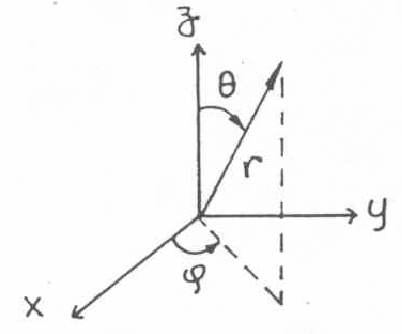
\includegraphics[width=2in]{images/qm/3DCS.png}
    \caption{Set-up of the 3D Coordinate System\label{3DCS}}
\end{figure}
\eqn{ \hat{L}_z = - i \hbar \ppphi }
\eqn{ \hat{L}^2 =  - \hbar^2 \left[ \frac{1}{\sin \theta} \pptheta \left( \sin \theta \pptheta \right) + \frac{1}{\sin^2 \theta} \ppphin2  \right] }

\subtopic{Define the Total Angular Momentum $\Jhat$}
We define the Total Angular Momentum as:
\eqn{ \Jhat = \Lhat + \Shat }
Notice we cannot solve for the three components of $\Jhat$ simultaneously neither, because: 
\eqn{ \left[ \Jhat_x, \Jhat_y \right] = i \hbar \Jhat_z,  \left[ \Jhat_y, \Jhat_z \right] = i \hbar \Jhat_x, \left[ \Jhat_z, \Jhat_x \right] = i \hbar \Jhat_y }


\subtopic{Eigenvalues of $\Lhat, \Jhat$}
See Liboff 9.3 for how we get the following equations: 
\eqn{ \boxed{ \hat{L}^2 \phi_{l,m} (\theta, \phi) = \hbar^2 l (l+1) \phi_{l,m} (\theta, \phi ), \fsp \fsp \hat{L}_z \phi_{l,m} (\theta, \phi) = \hbar m \phi_{l,m} (\theta, \phi ) } }
in which $l = 0,1,2, \cdots, m = -l, -l+1, \cdots, 0, \cdots l$. If we solve for $\hat{L}_x$ or $\hat{L}_y$ instead we will reach the same results as above. 

Similarly $\Jhat$ would give us:
\eqn{  \Jhat^2 \phi_{l,m} (\theta, \phi) = \hbar^2 j (j+1) \phi_{l,m} (\theta, \phi ), \fsp \fsp \Jhat_z \phi_{l,m} (\theta, \phi) = \hbar m_j \phi_{l,m} (\theta, \phi )  }
in which $j = 0,1/2,1,3/2,2, \cdots, m = -j, \cdots, j$. If we solve for $\Jhat_x$ or $\Jhat_y$ instead we will reach the same results as above. 

\subtopic{Eigenfunctions $\phi_{l,m}$ is Spherical Harmonics $Y_l^m(\theta, \phi)$}
The eigenfunction in the above equation, $\phi_{l,m}$, are commonly called the \textbf{Spherical Harmonics $Y_l^m (\theta, \phi)$}:
\eqn{ Y_l^m (\theta, \phi) = \frac{1}{\sqrt{2 \pi}} e^{im\phi} P_l^m (\phi)   }
A couple of things about the Spherical Harmonics:
\begin{itemize}
\item $\psi( r, \theta, \phi) = R(r) Y_{lm} (\theta, \phi)$. 
\item $\int_0^{2\pi} \dphi \int_0^{\pi} \sin \theta \dtheta |Y_{lm} (\theta, \phi) |^2 = 1.$
\item Spherical Harmonics also implies that the unit of angular momentum is $\hbar$.
\item Degeneracy: \textbf{For a given $l$ value, there are $2l+1$ number of degeneracy.} For instance, for $l=5$, we have 11 eigenstates $Y_5^5, Y_5^4, \cdots Y_5^{-5}$ that correspond to the same $l$, or the same $L^2 = 30 \hbar^2$. That is, for the same $L^2$, the projection onto the azimuthal plan are degenerate.  
\item $L_z$ is not continuous. Given a $L^2$, we can draw a bunch of cones, each surface describe the superposition of possible eigenfunctions. L will never entirely align with the z axis. 
\end{itemize}

\end{document}
